\documentclass[12pt,a4paper]{article}
\usepackage{lmodern}

\usepackage{placeins}
\usepackage{booktabs}
\usepackage{amssymb,amsmath}
\usepackage{ifxetex,ifluatex}
\usepackage{fixltx2e} % provides \textsubscript
\ifnum 0\ifxetex 1\fi\ifluatex 1\fi=0 % if pdftex
  \usepackage[T1]{fontenc}
  \usepackage[utf8]{inputenc}
\else % if luatex or xelatex
  \ifxetex
    \usepackage{mathspec}
    \usepackage{xltxtra,xunicode}
  \else
    \usepackage{fontspec}
  \fi
  \defaultfontfeatures{Mapping=tex-text,Scale=MatchLowercase}
  \newcommand{\euro}{€}
\fi
% use upquote if available, for straight quotes in verbatim environments
\IfFileExists{upquote.sty}{\usepackage{upquote}}{}
% use microtype if available
\IfFileExists{microtype.sty}{%
\usepackage{microtype}
\UseMicrotypeSet[protrusion]{basicmath} % disable protrusion for tt fonts
}{}
\usepackage[lmargin = 3 cm,rmargin = 2.5cm,tmargin=2.5cm,bmargin=2.5cm]{geometry}

% Figure Placement:
\usepackage{float}
\let\origfigure\figure
\let\endorigfigure\endfigure
\renewenvironment{figure}[1][2] {
    \expandafter\origfigure\expandafter[H]
} {
    \endorigfigure
}

%% citation setup
\usepackage{csquotes}

\usepackage[backend=biber, maxbibnames = 99, style = apa]{biblatex}
\setlength\bibitemsep{1.5\itemsep}
\addbibresource{R_packages.bib}
\bibliography{references.bib}
\usepackage{graphicx}
\makeatletter
\def\maxwidth{\ifdim\Gin@nat@width>\linewidth\linewidth\else\Gin@nat@width\fi}
\def\maxheight{\ifdim\Gin@nat@height>\textheight\textheight\else\Gin@nat@height\fi}
\makeatother
% Scale images if necessary, so that they will not overflow the page
% margins by default, and it is still possible to overwrite the defaults
% using explicit options in \includegraphics[width, height, ...]{}
\setkeys{Gin}{width=\maxwidth,height=\maxheight,keepaspectratio}
\ifxetex
  \usepackage[setpagesize=false, % page size defined by xetex
              unicode=false, % unicode breaks when used with xetex
              xetex]{hyperref}
\else
  \usepackage[unicode=true, linktocpage = TRUE]{hyperref}
\fi
\hypersetup{breaklinks=true,
            bookmarks=true,
            pdfauthor={Nils Paffen},
            pdftitle={Males, Catch Up!},
            colorlinks=true,
            citecolor=blue,
            urlcolor=blue,
            linkcolor=magenta,
            pdfborder={0 0 0}}
\urlstyle{same}  % don't use monospace font for urls
\setlength{\parindent}{0pt}
\setlength{\parskip}{6pt plus 2pt minus 1pt}
\setlength{\emergencystretch}{3em}  % prevent overfull lines
\setcounter{secnumdepth}{5}

%%% Use protect on footnotes to avoid problems with footnotes in titles
\let\rmarkdownfootnote\footnote%
\def\footnote{\protect\rmarkdownfootnote}

%%% Change title format to be more compact
\usepackage{titling}

% Create subtitle command for use in maketitle
\newcommand{\subtitle}[1]{
  \posttitle{
    \begin{center}\large#1\end{center}
    }
}

\setlength{\droptitle}{-2em}
  \title{Males, Catch Up!}
  \pretitle{\vspace{\droptitle}\centering\huge}
  \posttitle{\par}
\subtitle{Replication and summarization of \textcite{brunello} findings}
  \author{Nils Paffen}
  \preauthor{\centering\large\emph}
  \postauthor{\par}
  \predate{\centering\large\emph}
  \postdate{\par}
  \date{today}

\usepackage{booktabs,array,dcolumn,threeparttable,caption, tabularx, ragged2e,eqparbox, siunitx, collcell, makecell}
\usepackage{booktabs}
\usepackage{longtable}
\usepackage{array}
\usepackage{multirow}
\usepackage{wrapfig}
\usepackage{float}
\usepackage{colortbl}
\usepackage{pdflscape}
\usepackage{tabu}
\usepackage{threeparttable}
\usepackage{threeparttablex}
\usepackage[normalem]{ulem}
\usepackage{makecell}

%% linespread settings

\usepackage{setspace}

\onehalfspacing

% Language Setup

\usepackage{ifthen}
\usepackage{iflang}
\usepackage[super]{nth}
\usepackage[ngerman, english]{babel}

%Acronyms
\usepackage[printonlyused, withpage, nohyperlinks]{acronym}
\usepackage{changepage}

% Multicols for the Title page
\usepackage{multicol}

\begin{document}

\selectlanguage{english}


%\maketitle

\begin{titlepage}
  \noindent\begin{minipage}{0.6\textwidth}
	  \IfLanguageName{english}{University of Duisburg-Essen}{Universität Duisburg-Essen}\\
	  \IfLanguageName{english}{Faculty of Business Administration and Economics}{Fakultät für Wirtschaftswissensschaften}\\
	  \IfLanguageName{english}{Chair of Health Economics}{Lehrstuhl für Wirtschaftswissenschaften}\\
  \end{minipage}
	\begin{minipage}{0.4\textwidth}
	  \begin{flushright}
  	  \vspace{-0.5cm}
      \IfLanguageName{english}{\includegraphics*[width=5cm]{Includes/duelogo_en.png}}{\includegraphics*[width=5cm]{Includes/duelogo_de.png}}
	  \end{flushright}
	\end{minipage}
  \\
  \vspace{0.5cm}
  \begin{center}
  \huge{Males, Catch Up!}\\
  \vspace{.25cm}
  \Large{Replication and summarization of \textcite{brunello} findings}\\
  \vspace{0.5cm}
  \large{Term Paper}\\
  \vspace{0.5cm}
  \large{  \IfLanguageName{english}{Submitted to the Faculty of \\ Economics  \\at the \\University of Duisburg-Essen}{Vorgelegt der \\Fakultät für Wirtschaftswissenschaften der \\ Universität Duisburg-Essen}\\}
  \vspace{0.75cm}
  \large{\IfLanguageName{english}{from:}{von:}}\\
  \vspace{0.5cm}
  Nils Paffen\\
  \end{center}
  %\vspace{2cm}
  \vfill
  \hrulefill

  \noindent\begin{minipage}[t]{0.3\textwidth}
  \IfLanguageName{english}{Reviewer:}{Erstgutachter:}
  \end{minipage}
  \begin{minipage}[t]{0.7\textwidth}
  \hspace{1cm}Norman Bannenberg (M.Sc)
  \end{minipage}

  \noindent\begin{minipage}[t]{0.3\textwidth}
  \IfLanguageName{english}{Deadline:}{Abgabefrist:}
  \end{minipage}
  \begin{minipage}[t]{0.7\textwidth}
  \hspace{1cm}30.09.2020
  \end{minipage}

  \hrulefill

  \begin{multicols}{3}

  Name:

  Matriculation Number:

  E-Mail:

  Study Path:

  Semester:

  Graduation (est.):
 
 
  \columnbreak

  Nils Paffen

  3071594
  
  nils.paffen@stud.uni-due.de

  M.Sc. Economics

  \nth{3}

  Winter Term 2021

	\end{multicols}

\end{titlepage}

\newgeometry{top=2cm, left = 5cm, right = 2.5cm, bottom = 2.5cm}


\pagenumbering{Roman}
{
\hypersetup{linkcolor=black}

\setcounter{tocdepth}{3}
\tableofcontents
}

\newpage
\listoffigures
\addcontentsline{toc}{section}{List of Figures}

%\newpage
\listoftables
\addcontentsline{toc}{section}{List of Tables}

\section*{List of Abbreviations}
\addcontentsline{toc}{section}{List of Abbreviations}

\begin{adjustwidth}{1.5em}{0pt}

\begin{acronym}[dummyyyy]
 \acro{LASSO}{Least Absolute Shrinkage and Selection Operator}
 \acro{pcr}{Principal Components Regression}
 \acro{RMSE}{Root Mean Squared Error}
 \acro{MAE}{Mean Absolute Error}
 \acro{SEM}{Single Electricity Market}
 \acro{I-SEM}{Integrated Single Electricity Market}
 \acro{EU}{European Union}
 \acro{DM}{Diebold-Mariano}


%Falls eine Abkürzung in der Mehrzahl nicht einfach auf "s" endet muss das speziell eingestellt werden.
% \acro{slmtA}{super lange mega tolle Abkürzung} %Einzahl
 %\acroplural{slmtA}[slmtAs]{super lange mega tolle Abkürzungen} %Mehrzahl
 \acro{dummyyyy}{dummyyy}
\end{acronym}

\end{adjustwidth}

\restoregeometry

\newpage
\pagenumbering{arabic}
\hypertarget{introduction}{%
\section{Introduction}\label{introduction}}

This term paper will focus on the summarization and replicated results
of \textcite{brunello}. The main idea of the paper is to show if
extending years of compulsory schooling has an effect on the
distribution of wages. Further findings might be that compulsory school
reforms significantly affect educational attainment, which holds in this
replication study for almost none quantile, since the given data does
not help to show the possible effect of the instrument years of
compulsory schooling . This term paper, is limited to the data of the
SHARE data set, compared to a mixed dataset consisting of a
\enquote{data{[}set{]} drawn from the 8th wave of the European Community
Household Panel (ECHP) for the year 2001, the first wave of the Survey
on Household Health, Ageing and Retirement in Europe, or SHARE, for the
year 2004, and the waves 1993 to 2002 of the International Social Survey
Program (ISSP)}\textcite{brunello}. Due to the latter difference,
replicated results differ heavily from those in the original paper. More
about this in the dicussion section. This paper will start with a
summary of the empirical model and the strategy the authors used,
followed by a short overview of the SHARE dataset. Afterwards the
replicated results limited to the latter dataset were presented and a
short comparison to the findings of \textcite{brunello} is included. A
discussion of the replicated results is followed by a conclusion section
which closes this term paper.

\hypertarget{empirical-model}{%
\section{Empirical Model}\label{empirical-model}}

The author of the original paper starts with an introduction to
schooling and the direct correlation on wages. They claim that the
individuals or their parents choose years of schooling to maximise
\begin{align}u\left(w_{i}, s_{i}\right)=\ln \left(w_{i}\right)-c\left(s_{i}\right)\end{align}
where \(w_i\) is interpreted as a function of \(s_i\)
(\(w_i = g(s_i)\)), \(s_i\) itself is defined as year of schooling,
\(c(s_i)\) is the cost of schooling, while the index \(i\) indicates the
individual. The optimal \(s_i\) is then given by the \(s_i\) which
satisfies the equation of the marignal costs and the (expected) marginal
benefits of schooling. The marginal costs rise in schooling, decrease in
cognitive ability \(a_i\) and are a function of extenal controls \(X_i\)
and \(z\)
\begin{align} mc\left(s_{i}\right)=r\left(X_{i}, z\right)+\theta s_{i}-\kappa .
a_{i}\end{align} Further the authors follow a Miniceria earnings
function
\begin{align}\ln\left(w_{i}\right)=\beta s_{i}+s_{i}\left(\lambda a_{i}+\phi u_{i}\right)+\gamma_{w} X_{i}+a_{i}+u_{i}\end{align}
where constant term is incldued in X, in the model of the replication
study a constant is added seperatly to the model, the variable
\(a \sim G_a(0,\sigma^2_a)\) (cognitive ability) is known to the
individuals at the time of their choice. Following the authors
interpretation \(u \sim G_u(0,\sigma^2_u)\) can be described as fortune
in the labour market and formally as an error term orthogonal to
ability. Besides, \(u_i\) hold an zero mean demand shock which is
correlated with relative productivity of jobs and skills. Equation (3)
shows that schooling influences the location, due to \(\beta*s_i\), on
one hand and on the other the scale of the earnings distribution,
through the interaction with ability and labour market fortune. Ability
influences the individual earnings through \(a_i\) in a direct way and
via its product with schooling. As mentioned in the beginning, optimal
schooling \(s_i^*\) needs to satisfy
\begin{align}mc(s_i) = mb(si)\end{align} where \(mb(s_i)\) is defined as
\begin{align} mb(s_i)= \beta + \lambda a_i \end{align} therefore
\(s_i^*\) can be written as
\begin{align} s_i^* = \frac{\beta - r(X_i, z_i)}{\theta} + \frac{\lambda  + \kappa}{\theta}*a_i \end{align}

When \(\lambda>0\) ability and schooling are complements and both can be
defined as substitues if \(\lambda<0\) holds. Further the authors assume
that \(1+ \phi s_i > 0\), which secures the endogenoues variable log
earnings are a (increasing or decreasing) monotonic function of the
labour market fortune variable \(u_i\). The authors propose an exactly
identified triangular model as in Chesher's approach (7) and (8) but
mention that the orthogonality condition for the consistency of the OLS
estimation of (3) fails if one cant appropriately control for ability.
In this case the triangular model can be explained as the following.
Assume that the earnings of an individual are correlated with their
educational level. Let this educational level in this model be defined
as years of schooling (s). Therefore we need an instrument which
correlates with the educational level measurement but not with the
earnings.

To solve the latter and thereby generate a consistent estimatator,
\textcite{brunello} propose a variable \(z\) that is corellated with
schooling but orthogonal to individual ability conditional on schooling
and orthognal to the endogenous variable of (8). The instrumental
variable in this model is years of compulsory schooling \(ycomp\). Taken
this into account the (exactly indentified triangular) model can be
expressed as :
\begin{align} \ln(w)&=\beta s+s(\lambda a+\phi u)+\gamma_{w} X+a+u \\
s&=\gamma_{s} X+\pi z+\xi a \end{align} with
\(\xi=(\lambda+\kappa) / \theta\) Let
\(\tau_{a}=G_{a}\left(a_{\tau_{a}}\right) \text { and } \tau_{u}=G_{u}\left(u_{\tau_{u}}\right)\),
where \(a_{\tau_{a}}\) and \(u_{\tau_{u}}\) are the \(\tau-\) quantiles
of the distributions of \(a\) and \(u\), respectively. Additionally
define \(Q_{w}\left(\tau_{u}\mid s,X,z\right)\) and
\(Q_{s}\left(\tau_{a}\mid X,z\right)\) as the conditional quantile
functions corresponding to log wages and years of education. To achieve
the recursive conditioning model one needs to compute the control
variates first. Step one is to estimate the conditional quantile
functions of schooling \(s\) and afterwards subtract the estimated
values of the specific quantile from years of schooling. Considering (8)
again and the fact that the model is exactly identified one only remains
with the value of ability at the specific quantile tau. Formally :
\begin{align}a\left(\tau_{a}\right)=s-\bar{Q}_{s}\left(\tau_{a}\mid X,z\right).\end{align}
Afterwards one adjusts the conditional quantile functions of \(ln(w)\)
with the control variate of (9) so that the residuals, orthogonal to
ability, of the estimated conditional quantile regression of \(ln(w)\)
yields to \(u(\tau_u)\) of the following regression equation :
\begin{align}
\tilde{Q}_w[\tau_u|X, s, a(\tau_a)] = \beta s + s(\lambda a(\tau_a) + \phi u(\tau_u)) + \gamma_w X + G_{a}^{-1}\left(\tau_{a}\right) + G_{u}^{-1}\left(\tau_{u}\right)
\end{align}

Now one can construct the parameter \(\Pi(\tau_a,\tau_u)\) which is a
matrix with the following structure : \begin{align} \Pi\left(\tau_{a},
 \tau_{u}\right)=\beta+\lambda G_{a}^{-1}\left(\tau_{a}\right)+\phi
 G_{u}^{-1}\left(\tau_{u}\right)
 \end{align} Due to recursive conditioning
\(Q_{s}\left(\tau_{a}\mid X,z\right)\) on
\(Q_{w}\left[\tau_{u}\mid X,z\right)\) one yields to the following model
: \begin{align} Q_{w}\left[\tau_{u}
 \mid Q_s\left(\tau_{a} \mid X, z\right), X, z\right]&=Q_s\left(\tau_{a}
 \mid X, z\right) \Pi\left(\tau_{a}, \tau_{u}\right)+\gamma_{w}
 X+G_{a}^{-1}\left(\tau_{a}\right)+G_{u}^{-1}\left(\tau_{u}\right)&  \\
 Q_{s}\left(\tau_{a} \mid X, z\right)&=\gamma_{s} X+\pi z+\xi
 G_{a}^{-1}\left(\tau_{a}\right) & 
 \end{align} A a two stage fit of the latter models then gives us the
coeficient of \(Q_s\left(\tau_{a}\mid X, z\right)\) After we plug this
into \(\Pi\left(\tau_{a},\tau_{u}\right)\) for the coefficient
\(\beta\). We will repeat this step for each quantile tau (0.1, 0.3,
0.5, 0.9) but always altering only the quantiles of either \(\tau{u}\)
of
\(Q_{w}\left[\tau_{u}\mid Q_s\left(\tau_{a} \mid X, z\right), X, z\right]\)
or \(\tau{a}\) of the parameter
\(Q_s\left(\tau_{a}\mid X, z\right) \Pi\left(\tau_{a}, \tau_{u}\right)\)
. Therebey the study observes in the first case the effect of how a
specific quantile \(\tau_a\) of
\(Q_s\left(\tau_{a}\mid X, z\right)\Pi\left(\tau_{a},\tau_{u}\right)\)
interacts with the entire distribution of the log hourly earnings ,
while the latter measure the effect of the different quantiles of the
ability distribution on the fixed \(\tau_u\) of the endogenous variable
\(ln(w)\). Integrating the key parameter
\(\Pi\left(\tau_{a},\tau_{u}\right)\) with respect to \(\tau_a\) results
in mean quantile treatment effects. The latter gives an overview of how
an individual with average abilites is rewarded for educatinal
attainment in the different quantiles of the labour market luck
distribution.

\hypertarget{empirical-strategy}{%
\section{Empirical Strategy}\label{empirical-strategy}}

The crucial change in the papers strategy is, compared to other papers
using the same instrument, is that the results are not limited to the
conditional but also support the unconditional effect (marginalized
effect) of the quantile regression which can be interpreted as OLS
results. The latter will be shown by the mean quantile treatment effect,
as described in the last section. Following \textcite{brunello} serveral
assumptions for correct identification have to be made, namely :

\begin{itemize}
\item Due to monotonicity, with respect to \textit{u} in (7) and \textit{a} in (8), individuals in a higher quantile of the labour market fortune recieve higher wages, will individuals with higher ability tend to stay longer in educational training;
\item Once the decision of schooling is made an individual can't foresee their future draw from the distribution of labour market fortune, but can form expectations about their draw;
\item the instrument ycomp (years of compulsory schooling) has a remote impact on the distribution of education or the attainment to the latter. The treatment is assigned quasi-randomly due to their date of birth, whithout any parental influence;
\item the variation in the timing of the implementation might vary between muncipalities in a country but this has no effect on the general education level
\item there is no other channel besides the individual's education level, how the educational reform influences the log wages, so they are excluded form the wage equation of the observables (7)
\end{itemize}

Pooling the data from all countries helps to support the instrument
ycomp, since more observations help to measure the effect more robustly.
Doing so one can exploit the fact that due to the different timings of
compulsory school reforms we exclude the possibilty of a specific cohort
helps the instrument to become more valuable. This summarization does
not include the table 1 of the paper which is only informative for the
fact that compulsory schooling reforms were introduced in different
years at each country. To create the post and pre-treatment sample-size
the reform dates of Table 1 from \textcite{brunello} were used, with the
excpetion of Germany. Since municipalities were not observed in the
SHARE dataset the mean of the reform date at each muncipality was used
to identify post and pre-treatment individuals. The latter choosing was
done with the distance between birth cohort \(b\) and cohort
\(\overline{b}_k\), while the latter is identifyed as the first cohort
potentially affected by the change in mandatory school leaving age in
country \(k\).

A first feeling for the effect of \(ycomp\) respectivly to the SHARE
data can be seen in Figure 1. The graph shows the longitudanal data of
individuals five years before until five years after the compulsory
school reform happend in the respective countrys.

\begin{figure}
\centering
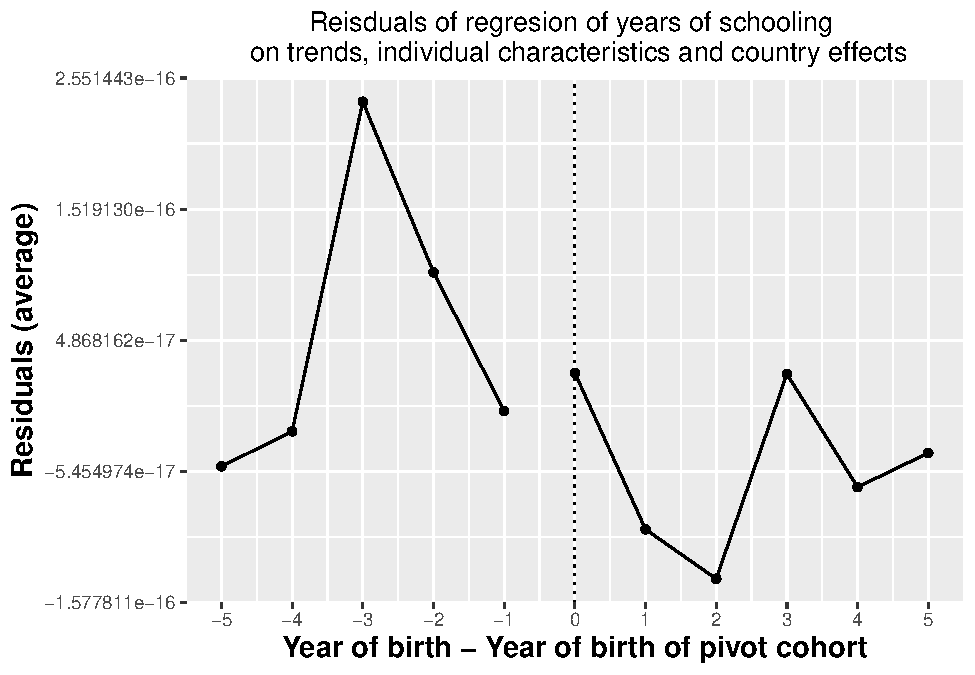
\includegraphics{term_paper_eem_files/figure-latex/unnamed-chunk-1-1.pdf}
\caption{\emph{The Effect of School Reforms on Educational Attainment}}
\end{figure}

\textit{Note}. The OLS gender-specififc regressions included a constant,
country dummies, \textit{q}, \textit{$q^2$} and their interactions with
country dummies and the GDP per head at the age when the pupil would
have finished compulsory schooling.

The residuals show that even this simple OLS regression produces results
with residuals which are more or less zero. This indicates that the OLS
model achieves to nearly perfectly explain the years of schooling. There
is even a downward jump when the reform hits the pupils. We will see in
latter results that in the first stage regression the instrument ycomp
is always insignificant and mostly negative.

\hypertarget{data}{%
\section{Data}\label{data}}

As mentioned in the beginning this recursive study is done using only
the data of the SHARE dataset. More than a decade has passed since the
paper of \textcite{brunello} was published. During this time the SHARE
data set of the first wave has been revised several times. In this term
paper the dataset of version 7.0\footnote{\url{https://releases.sharedataportal.eu/releases}}
is used. There is a more actual version, namely 7.1, but the STATA data
of this version are saved as .dat files and the .sav files of the 7.0
version were easier to implement. As mentioned in the empirical strategy
\textcite{brunello} uses several controls to claim that their results
are exactly identified. Attempts to gain access to these controls worked
only partly. Therefore the GDP and their first lags, as reported in the
Empirical strategy section, were retrieved from the OECD\footnote{\url{https://stats.oecd.org/viewhtml.aspx?datasetcode=PRICES_CPI\&lang=en\#}}.
All other controls were either not avaiable or did not match the
required time-length. The dataset is restricted to individuals aged
between 26 to 65, following the argument of \textcite{brunello} that
educational attainment does ot change after age 25. The final sample
contains 7165 observations from 10 countries instead of 12 of the
original paper.

\newcommand{\range}[1]{\eqparbox{ra}{#1}}
\newcolumntype{R}{>{\collectcell\range}c<{\endcollectcell}}



\begin{table}[!htbp]
\setlength\tabcolsep{3pt}
\sisetup{table-format=1.3, table-number-alignment=center}
\centering
\caption{Means of the key variable\strut} \label{}
\small
\begin{tabular}{@{} l SS[table-format=2.3]SRS[table-format=2.3]SS[table-format=4]S @{}}
\toprule
Country & {log w} & {s} & {ycomp} & \multicolumn{1}{c}{\makecell{Change in yrs.\\ of comp. school}}
 & {Age} & {\makecell{\%\\ Males}} & {Nobs} & {\makecell{\%\\ Complier}} \\
\midrule 
Austria & 2.022 & 12.632 & 8.679 & 8 to 9 & 55.368 & 0.526 & 209 & 0.679 \\ 
Belgium & 2.288 & 12.162 & 8.005 & 8 to 12 & 53.234 & 0.543 & 877 & 0.001 \\ 
Denmark & 2.973 & 13.523 & 7.115 & 7 to 9 & 54.592 & 0.489 & 681 & 0.057 \\ 
France & 2.401 & 11.303 & 8.64 & 8 to 10 & 53.328 & 0.474 & 878 & 0.32 \\ 
Germany & 2.58 & 14.705 & 8.7 & 8 to 9 & 55.309 & 0.51 & 857 & 0.7 \\ 
Greece & 2.038 & 12.22 & 6.021 & 6 to 9 & 54.182 & 0.617 & 708 & 0.007 \\ 
Italy & 2.196 & 10.066 & 7.112 & 5 to 9 & 55.606 & 0.601 & 411 & 0.528 \\ 
Netherlands & 2.748 & 13.289 & 9.02 & 9 to 10 & 54.69 & 0.535 & 910 & 0.02 \\ 
Spain & 2.597 & 12.766 & 6.04 & 6 to 8 & 56.396 & 0.46 & 1251 & 0.02 \\ 
Sweden & 2.039 & 9.487 & 8.454 & 8 to 9 & 55.355 & 0.567 & 383 & 0.454 \\ 
\bottomrule
\end{tabular} 
\end{table} 

Table 1 shows the log hourly real earnings, years of schooling, years of
compulsory schooling, average age and percentage of males. Education
attainment is highest in Germany (14.705) and lowest in Sweden (9.487).
Average age is highest in Spain (56.396) and lowest in Belgium (53.234).
Compared to the results of the paper by \textcite{brunello} the table is
extended by the column \textit(\% Complier) which indicates how many
individuals of the sample took the treatment and the column
\enquote{Change in years of comp. school} of Table 1 from
\textcite{brunello}. The latter columns indicate that the SHARE dataset
contains mostly people which where not affected by the reforms. This
might be a first explantion why the residuals of Figure 1 do not show
the results \textcite{brunello} found in their study. The reason might
be lack of observed treated individuals. For Belgium in the SHARE
dataset this is roughly around 0.1 \% of all individuals. Keeping in
mind, that Belgium was one of the last countrys to extend the years of
compulsory schooing, this might be also an answer to the question, why
the average age of Belgian individuals in this replication study differ
that much from the average age of the original paper. To capture
trend-like changes in the log earnings the study chooses, as described
in the original paper, a second order polynomial in \textit{q =t+7},
where t describes the distance between the individual and the first
cohort affected by the reform, and the effect of the interactions with
country specific dummies. This study follows the market-entry approach,
which matches each individual with the first lags of their country
specific GDP at that time when they would have applied to the job market
for the first time without the reform. So a Spanish citizen born in
1960, where the cirtical age before the reform was 12 would be matched
with the GDP values around 1972 to control for the posibility that the
changes in educational attainment after the reform can be credited to
the reform itself and not to some other economic time and/or
country-specific factors.

\hypertarget{empirical-evidence}{%
\section{Empirical Evidence}\label{empirical-evidence}}

Before this paper starts with the discussion of the results, one problem
that arised during almost all regression results that will follow in
this chapter is singular matrices. A square matrix can be described as
singular, that is, its \textit{determinant} is zero, in other words, one
or more of its rows(columns) can be exactly expressed as a linear
combination of all or some or some other its rows (columns). In the
multivariate data case, like the one in this paper, this can happen if
there are linear interdependances among the variables. Since
\textcite{brunello} adds many dummy variables it is possible to run into
this problem when your dataset is smaller, as in the reproduction
studies case. There are several ways to fix this problem such as
covariate reduction techniques such as LASSO, which only keeps variables
which are signifcant for the regression. The latter is explicitly
usefull if you have more variables than observations. But this does not
reflect this papers case. Another way to at least solve the problem of
exact linear combination is jittering. This means nothing else than a
small \textit{noise} is added to all values. In this paper the noise
level is a random value chosen from the interval \([-0.1;0.1]\) for each
value of the dataset. If this value is \textit{small} the interference
of the results is negligible.

As in the paper by \textcite{brunello} the first relationship presented
in this paper will be the quantile effect of education, as expressed by
years of schooling, on the log earnings, under the condtion that
education is treated as exogenous.


\begin{table}[!htbp]
\captionsetup{labelsep=newline, justification=centering}
  \begin{threeparttable}
       \caption{\textit{Quantile Effects When Education is Treated as Exogenous} \\
    \scriptsize (Sample size : 7,165) By gender (3,735 males and 3,430 females)}
     \begin{tabular}{*{6}{l}}
        \toprule
         & \( \tau=0.10\) & \( \tau= 0.30\) & \( \tau= 0.50\) & \( \tau= 0.70\) & \( \tau= 0.90\) \\
        \midrule
        \addlinespace
        \textit{Males}   & $\underset{(0.0025)}{0.0093^{***}}$ & $\underset{(0.0052)}{0.0088^{*}}$ & $\underset{(0.0048)}{0.0212^{***}}$ & $\underset{(0.0056)}{0.0331^{***}}$ & $\underset{(0.0085)}{0.0294^{***}}$
\\
        \textit{Females}& $\underset{(0.0025)}{0.0065^{***}}$ & $\underset{(0.0052)}{0.0148^{***}}$ & $\underset{(0.0048)}{0.0238^{***}}$ & $\underset{(0.0056)}{0.0291^{***}}$ & $\underset{(0.0085)}{0.0233^{***}}$ \\
        \bottomrule
     \end{tabular}
    \begin{tablenotes}[flushleft]
      \small
      \item \textit{Note.} Each regression included a constant, country dummies, \textit{q}, \textit{$q^2$} and their interactions with country dummies, age, age squared, and the GDP per head at the age when the pupil would have finished compulsory schooling. $\tau$ denotes the quantile of the distribution of wages. Three stars, two stars and one star for statistically significant coefficients at the 1\%, 5\% and 10\% confidence level. Bootstrapped standard errors are shown in parentheses.
    \end{tablenotes}
  \end{threeparttable}
\end{table}

Table 2 highlights returns to a one year increase in education from the
10th to the 90th quantile. All results are statistically significant at
the highest level. In difference to \textcite{brunello} the returns for
males are mostly higher than those for females. The latter beats the
other gender only in the 30th and 50th quantile. Following this results
the 90-10 log wage differential would indicate that one additional year
of education lead to an increase of 2.02 percantage points for males and
an increase of 1.67 for females. These results draw a picture of a world
where the males need to catch up to their gender counterpart. Besides
that, the results look robust and as expected, since in this model the
instrument does not play any role in the causal inference of log
earnings.

As argued by \textcite{brunello} we can't treat education as exogenous
since we expect a correlation between the log earnings and the latter.
Therefore we will use the described instrument ycomp to explain
schooling and use these values as a substitute for education in our log
earnings regression model.


\begin{table}[!htbp]
\captionsetup{justification=centering}
  \begin{threeparttable}
       \caption{\textit{First Stage Effect of ycomp on s} (Sample size : 7,165)}
        \begin{tabular}{*{6}{l}}
        \toprule 
        \textit{Males}  & \( \tau_a=0.10 \) & \( \tau_a= 0.30 \) & \( \tau_a= 0.50 \) & \( \tau_a= 0.70 \) & \( \tau_a= 0.90 \) \\
        \midrule     \\
        Coeff. (s.e.)   & $\underset{(0.0872)}{-0.0049}$ & $\phantom{-}\underset{(0.1814)}{0.2409}$ & $\phantom{-}\underset{(0.1656)}{0.0722}$ & $\phantom{-}\underset{(0.2665)}{0.1098}$ & $\phantom{-}\underset{(0.1662)}{0.0515}$    \\
        F-test (p-value) & $\phantom{-}\underset{(0.304)}{1.057}$ & $\phantom{-}\underset{(0.56)}{0.3398}$ & $\phantom{-}\underset{(0.9355)}{0.0065}$ & $\phantom{-}\underset{(0.6495)}{0.2065}$ & $\phantom{-}\underset{(0.724)}{0.1247}$\\
        \midrule 
        \textit{Females}  & \( \tau_a=0.10 \) & \( \tau_a= 0.30 \) & \( \tau_a= 0.50 \) & \( \tau_a= 0.70 \) & \( \tau_a= 0.90 \) \\
        \midrule \\
        Coeff. (s.e.)    & $\phantom{-}\underset{(0.1373)}{0.0094}$ & $\underset{(0.2112)}{-0.0248}$ & $\phantom{-}\underset{(0.1556)}{0.0669}$ & $\phantom{-}\underset{(0.1799)}{0.0994}$ & $\underset{(0.2008)}{-0.0054}$  \\
        F-test (p-value) & $\phantom{-}\underset{(0.3545)}{0.8576}$ & $\phantom{-}\underset{(0.6941)}{0.1547}$ & $\phantom{-}\underset{(0.3688)}{0.808}$ & $\phantom{-}\underset{(0.3564)}{0.8507}$ & $\phantom{-}\underset{(0.4508)}{0.5689}$ \\
        \bottomrule
     \end{tabular}
    \begin{tablenotes}[flushleft]
      \small
      \item \textit{Note.} See Table 3. $\tau_a$ denotes the quantile of the distribution of ability.
    \end{tablenotes}
  \end{threeparttable}
\end{table}

In the section about the empirical strategy we already got a feeling for
the effect of the instrument ycomp. Figure 1 shows almost zero residuals
which indicates that it is likely that another coefficient doesn't add
any significant value to explain the years of schooling. The results in
Table 3 match these expactions. Given the SHARE dataset, the
instrumental variable \textit{ycomp} is insignificant at all quantiles
for both genders. Besides, this step it is important to analyze if our
instrument is a valid instrument. Using the Stock and Staiger rule of
thumb, a selected instrument apears to be a weak instrument if the
F-test for it's inclusion is lower than 10. The results, again for both
genders, clearly show that the instrument is weak and that all F-tests
appear to be insignifcant.\footnote{Typically those results should lead
  the model designer to a reconsideration of either the model, the
  strategy, the data or all three of them. Since this study just
  replicates the results, given the limitations of the dataset SHARE,
  this paper continues to discuss the reproduced findings and ignores
  the obvious warning signs the latter results show.} Under condition
that those result would be representative, males at the 10th quantile of
the distribution would face a slight decrease in educational attainment
around -0.5\% per extra year of compulsory schooling while females at
the same quantile would face an increase of roughly 1\% in educational
attainment per extra year of compulsory schooling.

In the next step


\begin{table}[!htbp]
\captionsetup{labelsep=newline, justification=centering}
  \begin{threeparttable}
       \caption{\textit{Quantile Effects When Education is Treated as Exogenous} \\
    \scriptsize (Sample size : 7,165) By gender (3,735 males and 3,430 females)}
     \begin{tabular}{*{6}{l}}
        \toprule 
        \textit{Males}  & \( \tau_u=0.10\) & \( \tau_u= 0.30\) & \( \tau_u= 0.50\) & \( \tau_u= 0.70\) & \( \tau_u= 0.90\) \\
        \midrule     \\
        $\tau_a = 0.1$    & $\phantom{-}\underset{(1.6418)}{18.5705^{***}}$ & $\phantom{-}\underset{(0.7968)}{7.9764^{**}}$ & $\phantom{-}\underset{(0.8622)}{7.5947^{**}}$ & $\phantom{-}\underset{(0.8778)}{11.1463^{***}}$ & $\phantom{-}\underset{(1.9126)}{7.6605}$  
\\
         $\tau_a = 0.3$   & $\phantom{-}\underset{(0.1817)}{0.7117}$ & $\phantom{-}\underset{(0.121)}{0.3057}$ & $\phantom{-}\underset{(0.1064)}{0.291^{*}}$ & $\underset{(0.1163)}{0.4272^{***}}$ & $\phantom{-}\underset{(0.2019)}{0.2936}$
\\
          $\tau_a = 0.5$    & $\phantom{-}\underset{(0.218)}{1.7513}$ & $\phantom{-}\underset{(0.1313)}{0.7522}$ & $\phantom{-}\underset{(0.1142)}{0.7161}$ & $\phantom{-}\underset{(0.1131)}{1.0512}$ & $\phantom{-}\underset{(0.1861)}{0.7224}$ \\
           $\tau_a = 0.7$   & $\phantom{-}\underset{(0.4483)}{1.8353}$ & $\phantom{-}\underset{(0.2273)}{0.7883}$ & $\phantom{-}\underset{(0.1914)}{0.7505^{**}}$ & $\phantom{-}\underset{(0.2551)}{1.1016^{***}}$ & $\phantom{-}\underset{(0.5155)}{0.7571}$  
           \\
           
           $\tau_a = 0.9$    & $\phantom{-}\underset{(0.4067)}{7.9706}$ & $\phantom{-}\underset{(0.2017)}{3.4235}$ & $\phantom{-}\underset{(0.1849)}{3.2593}$ & $\phantom{-}\underset{(0.2211)}{4.7841^{***}}$ & $\phantom{-}\underset{(0.4422)}{3.2879^{***}}$ 
\\ 
Mean effect+ &6.167885 & 2.649243 & 2.522340 &  3.702072 &  2.544303
\\ \toprule
        \textit{Females} &  \( \tau_u=0.10\) & \( \tau_u= 0.30\) & \( \tau_u= 0.50\) & \( \tau_u= 0.70\) & \( \tau_u= 0.90\) \\
        \midrule
        \addlinespace
        $\tau_a = 0.1$ & $\underset{(0.3065)}{-0.0087}$ & $\phantom{-}\underset{(0.1816)}{0.5695}$ & $\phantom{-}\underset{(0.1924)}{0.5237}$ & $\phantom{-}\underset{(0.2308)}{0.3996}$ & $\phantom{-}\underset{(0.3037)}{1.0701}$   \\
         $\tau_a = 0.3$   & $\underset{(1.3782)}{-0.414}$ & $\phantom{-}\underset{(0.9251)}{26.9564}$ & $\phantom{-}\underset{(0.8135)}{24.7813}$ & $\phantom{-}\underset{(1.0035)}{18.9156}$ & $\phantom{-}\underset{(1.605)}{50.6541}$ \\
          $\tau_a = 0.5$   & $\underset{(0.2067)}{-0.0047}$ & $\phantom{-}\underset{(0.1105)}{0.3051}$ & $\phantom{-}\underset{(0.1073)}{0.2806}$ & $\phantom{-}\underset{(0.1191)}{0.2141}$ & $\underset{(0.1873)}{0.5733}$   \\
           $\tau_a = 0.7$   &  $\phantom{-}\underset{(0.268)}{0.0131}$ & $\underset{(0.1233)}{-0.8538}$ & $\underset{(0.1268)}{-0.785}$ & $\underset{(0.1534)}{-0.5991}$ & $\underset{(0.219)}{-1.6043}$    \\
           $\tau_a = 0.9$    & $\phantom{-}\underset{(0.2297)}{0.0258}$ & $\underset{(0.1146)}{-1.6797}$ & $\underset{(0.1094)}{-1.5445}$ & $\underset{(0.1335)}{-1.1786^{*}}$ & $\underset{(0.1889)}{-3.1563}$    \\
           Mean effect+ & -0.07770027 &  5.05951296 & 4.65119676 &  3.55031764 & 9.50738651 \\
        \bottomrule
     \end{tabular}
    \begin{tablenotes}[flushleft]
      \small
      \item \textit{Note.} See Table 
    \end{tablenotes}
  \end{threeparttable}
\end{table}

the full matrix of quantile treatment effects is estimated by applying
the control variate approach as described by \textcite{MaKoenk} in the
sense of \textcite{brunello}. The results can be seen in Table 4. As
expected through the results given by the first stage in Table 3, most
of the coefficients are insignificant and or unlikely high. Examples are
the 10th and 90th quantile for males of \(\tau_a\) when \(\tau_u\) and
the 30th quantile for females.

In compariso \textcite{brunello} finds that the estimated increase in
earnings for males at the lowest quantile are 7.48\% compared to roughly
1800\% in the result of the replication study and stay at a very high
percantage level for mostly around 700\% to 800\% percent. The page for
the females looks quite the opposite. It seems that, again, males have
to catch up extremly since many of the results from the bottom to the
highest quantile of ability show some negative coefficients. But there
are some mentionable positive results for the latter gender, too. The
findings would expect the estimated returns of education of females
which find themselves in the 30th quantile of the ability distribution
and the highest quantile of the labour market luck distribution of
roughly 5000\%. If the latter would be the case we would expect much
more women from the lower ability distribution to earn a fortune after
leaving school with an extra year of education while hitting the jackpot
in the \enquote{labour market luck lottery} aka presenting an indivdiual
in the 90th percentile of the labor market fortune distribution.

In a more realistic world presented by the results of
\textcite{brunello} females are thoses to catch up at the fight for
wages. The authors found that especially women from the lowest
percentile benefit from an extra year of compulsory schooling which is
expressed as returns for the surplus education of roughly 10\%.

\hypertarget{discussion-of-the-findings}{%
\section{Discussion of the findings}\label{discussion-of-the-findings}}

Either the quantile regression method fails completly on this kind of
dataset or the dataset is not good to show the effect of the chosen
treatment \textit{ycomp}. \textcite{brunello} add in their section about
robustness checks that it is likely that an measurement error of the key
models ((7) and (8) in this paper and (6) and (7) in
\textcite{brunello}) occurs but not for the ECHP data, \enquote{because
years of education are computed there by using the information on the
age when full time education was stopped}. Since this study only uses
the data given by the SHARE study, it is possible that the erroneous
looking results of this replication might be biased due to this problem.
\textcite{brunello} further add that another bias in their results might
be due to lack of controls for parental background, which they try to
control for by using the unenmployment rate, which isn't avaiable for
this replication, and the GDP per capita. They argue that other
explanations like easier access to credit funds or higher education of
the parents could give the treated individuals an unobserved exogenous
boost which might be falsly captured by ability. The key problem of this
replication study seems to be the SHARE dataset. Rembering the results
of Table 1, one can easily see that many of the individuals are not
accounted as compliers. For example, Spain, which is the country where
most individuals come from, compared to all other countries, has a rate
of only 2\% of individuals affected by the instrument. The Netherlands
show the same qoute and being the second highest country in terms of
share of observed individuals. Greece, Belgium and Denmark show extremly
low compliance rates aswell. Given these numbers it should be no
surprise that the instrument is never significant due to lack of
observed treated individuals. An plausible explanation why
\textcite{brunello} added these data to their study, might be as mostly
control individuals for the treatment effect.

\hypertarget{conclusions}{%
\section{Conclusions}\label{conclusions}}

The results of the replication study shed light on how returns of
compulsory schooling to both genders affects their earnings. Mostly for
men in a positive manner while their gender counterpart should leave
school as early as possbile since in the world of the replicated results
women even lose if they stay in school much longer than needed. The
latter does not hold for those women of the 30th quantile of the ability
distribution. Further attempts to replicate the results of
\textcite{brunello} and to achieve plausible results are highly
encouraged to not limit their study to only the SHARE dataset.

\newpage

\printbibliography



\end{document}
